\section{Scene Distance Measure}
\label{sec:Scene Distance Measure}

The purpose of this experiment is to investigate the range of distance measure scores from our training data in Section \ref{sec:Field of View}. Figure \ref{fig:scene-distance-measure} illustrates the average distance measure score for each algorithm from our dataset, comparing different and same scenes. The scenes were labeled according to our binary labeling system, where one indicates similar scenes and zero otherwise. The graph also includes the standard error above and below the mean distance measure, indicating the range within which the true mean distance measure score is expected. This graph mirrors the same experiment performed by Pop-Share. Pop-Share's training data was much more diverse, with around 16 hours of raw video spanning across various environments and recorded from many devices. GhostPeerShare was training on a total of 100 minutes of indoor video data recorded by two phones.

\begin{figure}[t]
    \centering
    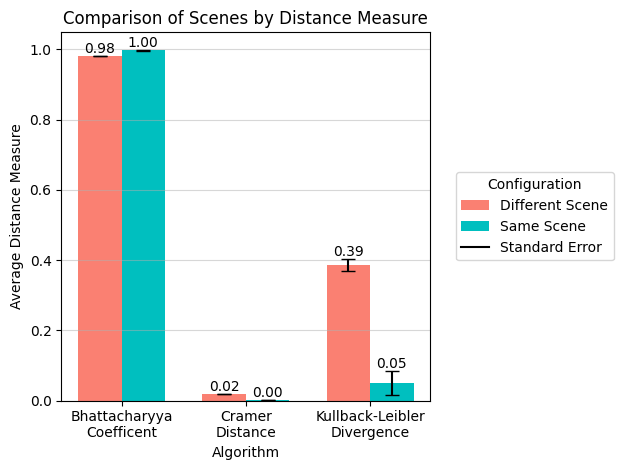
\includegraphics[width=0.8\textwidth]{5 Results/Figures/5.4 Bar Chart.png}
    \caption{Scene Distance Measure}
    \label{fig:scene-distance-measure}
\end{figure}

For the Bhattacharyya Coefficient, a perfect score of 1.00 indicates that the two scenes are identical, while a score of zero denotes no overlap. From Pop-Share, the same pattern was found for the Bhattacharyya Coefficient, containing little variance between different and same scenes and significantly less standard error than other metrics. In our experiments, we observed a 0.02 variance between the distance measures for different and same scenes. This minimal variance is likely attributed to the uniformity of the scene types recorded, as both sets were filmed indoors, and the fact that the same devices were used during the experiments, which limited the diversity in the captured footage.

For Cramer Distance, a perfect score of 0.00 indicates that the two scenes are identical, while a score of 1.0 is the maximum distance between two probability distributions. From Pop-Share, Cramer Distance contained a significant absolute difference of around 0.25 between different and same scenes. In our experiments, we observed significantly less variance, 0.02, between the distance measures for different and same scenes. The lack of variance is likely attributed to the limited data used in our experiments compared to Pop-Share. 

For the Kullback-Leibler Divergence (KLD), a perfect score of 0.00 indicates that two scenes are identical, while the upper limit is infinity; the smaller the score, the more similar the two probability distributions are. From Pop-Share, KLD was the leading indicator of dissimilarity, however, their experiments contained significant variance greater than 1 between different and same scenes. In our experiments, we observed a 0.34 variance between the distance measures for different and same scenes. This represents the highest variance observed among all of our distance measures and serves as a significant indicator that two scenes may be different.

The key takeaway from our experiments is that while the individual scores for the distance measures exhibit minimal variance, they still effectively differentiate between similar and different scenes. This consistency suggests that the implemented algorithms can reliably assess similarity, even in scenarios where the overall variation in scores is low. Consequently, the results highlight the robustness of our methodology in accurately identifying scene differences, which is crucial for applications requiring precise content analysis without revealing the underlying video data.
